\documentclass{article}

\usepackage{graphicx}
\usepackage{hyperref}

\title{HackPSU RFID Scanner Box User Manual}
\date{\today}
\author{ \href{mailto:technology@hackpsu.org}{HackPSU Technology Team}}

\begin{document}
\maketitle

\section*{Introduction}
This document serves as the reference manual for the HackPSU RFID scanner box.  This manual does not detail the implementation of the device; the intention of this document is to provide a user with the necessary information to operate the scanner and to troubleshoot some basic problems. 

\tableofcontents

\section{RFID Devices}
This scanner uses the MFRC522 RFID transceiver unit. The present implementation is intended for use with MIFARE compatible RFID devices.  This decision was made to simplify the implementation of the scanning functionality.  Other devices may be compatible, but may not work.  It is suggested that each operator have a wristband with a valid UID and the MASTER\_KEY from the configuration to unlock the box to aid in debugging possible issues.

\section{Keypad Controls}
The keypad behaves like a normal numeric keypad in most cases; however, the nonnumerical characters have special functions listed below.  
\begin{itemize}
	\item[\textbf{A}] The 'A' key acts as a scroll up function in all menus.
	\item[\textbf{B}] The 'B' key acts as a scroll down function in all menus, and the 'B' key acts as the back key when in a non-menu state, returning the user to the main menu.
	\item[\textbf{C}] The 'C' key serves no special functionality presently.  In a future implementation, it will scroll the LCD.
	\item[\textbf{D}] The 'D' key transitions the box into the locked state.
	\item[\textbf{*}] The '*' key acts as a clear or negative input button.  
	\item[\textbf{\#}] The '\#' key acts as a submit or positive input button.
\end{itemize}

\section{Access Control}
Access control is handled in a locked state, where the scanner waits for a staff wristband to be scanned.  This is intended to provide a minimal layer of security on the device so that event goers cannot scan themselves into events.  The duplicate state will produce a staff band by writing the master key into the data sector of the band.  Access control can be disabled in the implementation.

\section{Scanning}
Upon entering the "Locate \& Scan" state, the scanner will fetch a list of available locations from the cache server defined in the configuration header.  To select an entry from the menu, press the '\#' key. Numerical inputs are not supported in this menu.  Once the location is selected; wristbands may be scanned.  The scanner is set with a timeout, which cycles the functionality to listen for keypad driven state transitions using the 'B' and 'D' keys.  Upon receiving a successful scan, a request is sent to the cache server to commit the scan.  If the response is received and the "isRepeat" field is set to 'false' then the LCD will display "Allow" if no response is received or if the field is set to 'true' then "Deny" will be printed to the LCD.  The only case where the "isRepeat" field will be set to 'true' is if the event at the current location is a 'food' event and the user has been scanned once before.  
\subsection{User Guide}
\begin{itemize}
	\item The box will fetch a list of active locations
	\item Select one location using the '\#' key and navigate the menu with 'A' and 'B' for up and down respectively.
	\item The box is now set to a location and is ready to scan
	\item Scan each entrant for the event, waiting for a response to be displayed in between scans
	\item The box will display "Allow" or "Deny" based on the validity of the scan
\end{itemize}
\subsection{Reasons for Denial}
\begin{itemize}
	\item The box will deny any user with an invalid RFID band; they must be checked in first
	\item The box will deny any user who attempts to cycle though a food event more than once
	\item The box should hang, but may deny a user if WiFi becomes disconnected or if the cache server is unavailable.
\end{itemize}

\section{Check-in}
The check-in state follows a linear flow.  First a pin must be entered using the keypad.  Once a pin is submitted, a request to retrieve the user data will be made.  If no response is received or if the pin is not found on the cache server, the message "Invalid Pin" will be displayed.  Upon successfully entering a pin, a new prompt will appear, asking the user to validate the name displayed below.  The user may press '\#' to confirm that the user pin was correct, or '*' to return to pin entry.  The user will then be prompted to scan a wristband.  If the wristband's UID already exists in the cache server's database, then a message instructing the user to dispose of the band will be displayed.  If the scan function times out before a wristband is scanned, the pin will need to be entered again. If the user name is confirmed and a wristband is scanned, the user will be checked-in on the cache server.  The next step displays the user's shirt size and asks for photo consent.  Any key can be pressed to escape the photo consent menu, although using '*' or '\#' is recommended as this may change in a future implementation.  The scanner will then return to the beginning of the check-in process.  Press 'B' or 'D' in the pin entry state to leave the check-in state. 
\subsection{User Guide}
\begin{itemize}
	\item The box will request that a registrant's pin is entered
	\item Use the keypad to enter the registrant's base 10 bin, or press 'D' to escape to the locked state
	\item If the registrant's pin was invalid, a message will be displayed
	\item If the registrant's pin was valid; it will ask that you confirm their name.  Use the '\#' key to confirm or the '*' key to deny
	\item Once the registrant's name is confirmed, the box will be ready to assign them a UID from a wristband
	\item Scan the wristband now, and if the box says to scrap the wristband, please discard the band as a UID collision has occurred
	\item Once the wristband has been successfully scanned, the registrant's shirt size will be displayed and a prompt asking for photo consent will appear.
	\item Photo consent is not handled by our cache or database server, so photo consent must be tracked physically.  Press any key to continue
	\item The box will now cycle back to the first step
\end{itemize}
\subsection{Reasons for Error}
\begin{itemize}
	\item "Invalid Pin" will be displayed if a user enters an invalid pin or a pin that has already registered pin.
	\item "Scrap Band" will be displayed if the given wristband or a wristband with the same UID has already been registered.  Please discard the wristband and try another one.
	\item Either of these error states may also be caused by a WiFi disconnect or by the cache server becoming unreachable.  Check that the WiFi is still connected in the WiFi status mode and validate that the cache server is still running at the correct address
\end{itemize}

\section{Configuration}
The configuration for the device must be done prior to deployment.  All configuration should be done in the sketch's hackPSUconfig.h file.  The following fields are available:
\begin{itemize}
	\item[\textbf{MASTER\_KEY}] This defines the key written to sector 4 of the staff wristbands used to unlock the scanner as well as the key that the duplicate state writes to staff bands.
	\item[\textbf{SCAN\_TIMEOUT}] The time that the scanner will block for when attempting to interact with a wristband.  
	\item[\textbf{BAUD\_RATE}] The baud rate for the serial communications.  
	\item[\textbf{WIFI\_CONSTS}] This definition should be empty; it is a flag marking whether or not the SSID and PASSWD fields have been defined; if unset, the sketch will fail to compile. 
	\item[\textbf{REDIS}] The address of the cache server; this should not have any protocol, just a network address and a port.
	\item[\textbf{SSID}] The name of the network to connect to; if this network cannot be found, the scanner will not boot.
	\item[\textbf{PASSWD}] The password for the network that is being connected to; if this is incorrect, the scanner will not boot.
	\item[\textbf{fp}] The fingerprint of the SSL certificate being used by the caching server.
\end{itemize}

\section{Troubleshooting}

\subsection{Failure to Scan an RFID Tag}
There are two reasons that the box may not scan an RFID Tag.  The most likely reason is that the given band was already scanned.  The scanner is stately and will prevent the same band from being scanned twice in a row.  This is done to prevent multiple unintentional scans, but may result in the scanner being soft locked.  To unlock the scanner, simply scan another wristband or enter the locked state.  It is suggested that each operator have a band with the MASTER\_KEY written to it to unlock the box from the locked state and to free the scanner from a soft lock.  

\subsection{Long Scan Times}
If scan times are taking a long time, the likely culprit is a bad RFID signal or a long RTT on the connection to the cache server.  A bad RFID signal may be caused by excess material between the wristband and the scanner of the box.  A long RTT can be caused by long network hops to the cache server or by network congestion.  To test RTT with your cache server, use the following "time\_total" feature in cURL. 

\subsection{Failure to Boot}
A failure to boot generally means that the network configuration is incorrect.  Double check the network SSID and password are correct.  If they are correct, the LCD should indicate that the network connection succeeded.  The next blocking call will be to get an API key from the cache server.  This call will fail if the cache server is misconfigured, or if the scanner is misconfigured.  On the scanner side, check that the address is correct and does not have "http://" or "https://" prepended to the hostname.  Also validate that the port on the server is correct.  The next point of failure will be in the SSL certificate fingerprint or if HTTPS is not implemented on the server, the implementation for the API wrapper must be changed to use HTTP instead of HTTPS.  \\
If the box fails reaches the point where it is locked and will not enter the menu state, the user must scan a wristband, which contains the master key value as defined in the configuration header.  If your wristbands do not support read/write access, undefine SECURE\_BOOT in the state machine header to bypass a secure boot.  

\subsection{Unexpected Shutdowns}
The scanner may crash and shutdown.  When this happens, the most common failure mode during developent was an unhanded exception like a memory allocation failure.  The scanner will attempt to reenter the program.  In this case, unplug the power and force the scanner to boot from the beginning.  \\
If the scanner shuts down unexpectedly, check its battery charge; the device does not know how much battery is left and will not give a low battery warning.  

\subsection{Soft Locked Scanner}
The scanner should not ever soft lock.  In the event that it does, the best option is to power cycle the device.  Another alternative would be to hold the 'B' or 'D' key and hope that the box times out and transitions to the menu or lock state.

\section{Appendix}

\subsection{Finite State Machine}
\begin{center}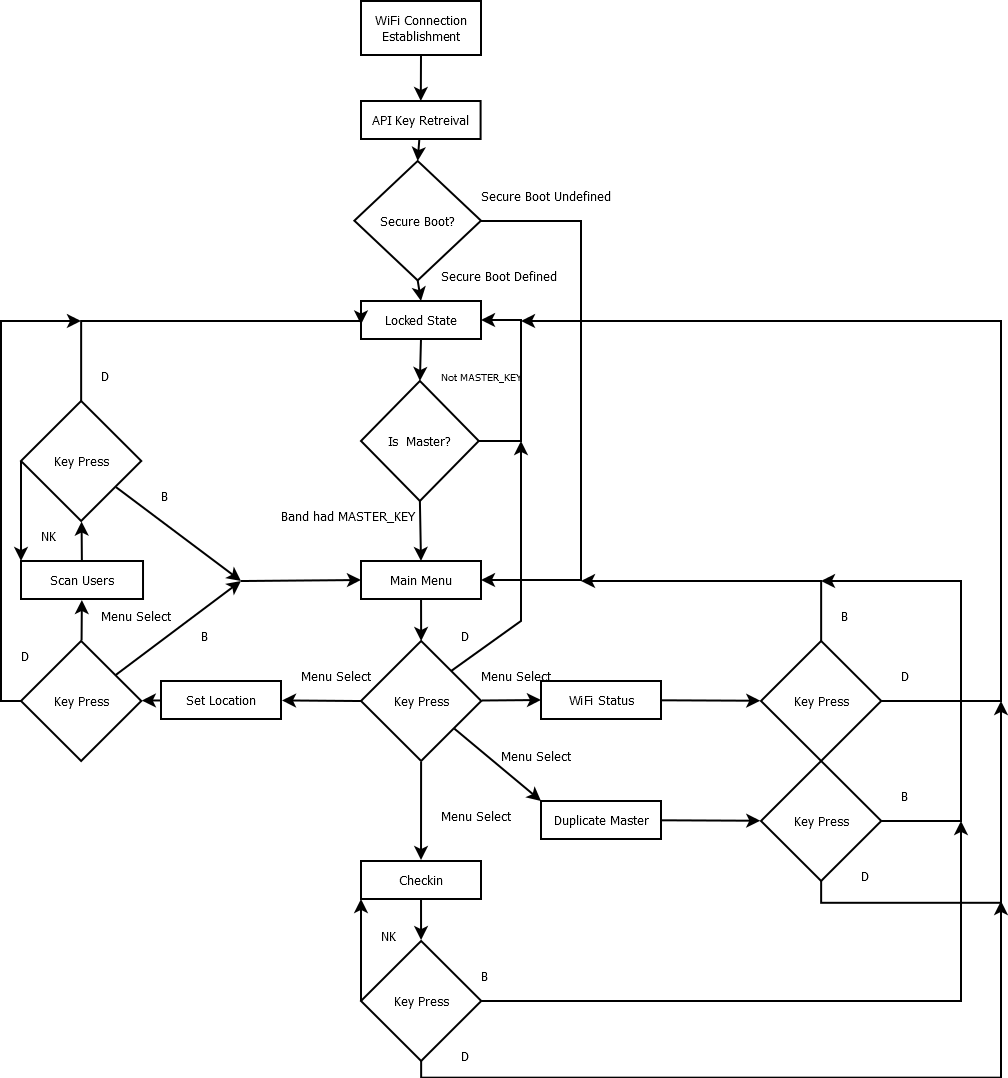
\includegraphics[scale=0.25]{states}\end{center}

\end{document}